\section{Evaluation}
\label{sec:eval}
In this section, we introduce the experimental setup
and analyze the performance of different models.

\subsection{Datasets}
CNN/Daily Mail~\citep{HermannKGEKSB15}
\footnote{\url{https://cs.nyu.edu/~kcho/DMQA/}} 
is a popular summarization dataset, 
which contains news articles paired with summaries.
There are 286,817 training pairs,
13,368 validation pairs and 11,487 test pairs.
\tabref{tab:example} shows an example pair from training data.
We follow \cite{SeeLM17} in data preprocessing and use 
the non-anonymized version, which fills in the blanks with answer named entities.

Also we tried our model on other two abstractive summarization datasets about news, which are Newsroom \citep{Newsroom18} and DUC 2002 \footnote{https://www-nlpir.nist.gov/projects/duc/guidelines/2002.html}. For Newsroom, there are 1,321,995 document-summary pairs, which are divided into training (76\%), development (8\%), test (8\%), and unreleased test (8\%). At testing, we use 8\% released test data. DUC-2002 (DUC) is a test set of document-summary pairs. We use the models trained on CNN/Daily Mail to do the test on DUC and demonstrate the generalization of the models.


\subsection{Model Parameters and Evaluation Metrics}
\label{sec:expset}
In the following experiments, 
we tokenize source documents and targets 
using the word tokenization method from NLTK (Natural Language Toolkit). 
The NLTK module is a massive toolkit, 
aimed at helping with the entire Natural Language Processing (NLP) methodology.
All the competing models contain $8$ convolutional layers in
both encoders and decoders, with kernel width of $3$.
For each convolutional layer, 
we set the hidden state size to $512$ and the embedding size to $256$.
To alleviate overfitting,
we apply a \textit{dropout} ($p=0.2$) layer to 
all convolutional and fully connected layers.
Similar to \citep{gehring2017convs2s},we use Nesterov's
accelerated gradient method \citep{SutskeverMDH13} with gradient clipping $0.1$ \citep{PascanuMB13}, momentum $0.99$,
and initial learning rate $0.2$.
Training terminates when learning rate $\le 10e$-$5$.
Beam size $b=5$ at test time.

We set the threshold $\beta$ to $3$, 
because nearly $90\%$ 
of sections are with length$>=$3.
We set $n$ (Equation (\ref{eq:s})) to $5$,
since less than $5\%$ of reference summaries have
the LCS of less than $5$.
We use the following evaluation metrics:
\itemsep0em
\begin{itemize}

\item \textbf{ROUGE} scores (F1), including ROUGE-1 (R-1), ROUGE-2 (R-2) and
ROUGE-L(R-L)~\citep{rouge-a-package-for-automatic-evaluation-of-summaries}.
ROUGE-1 and ROUGE-2 respectively refer to the overlap of unigram (each word) and bigrams between the generated summaries and reference summaries.
ROUGE-L denotes Longest Common Subsequence (LCS) based statistics.
ROUGE-2 is the most popular metric for summarization.

\item \textbf{Repeatedness} (Rep) 
includes N-gram repeatedness, sentence repeatedness
and total repeatedness.
\begin{itemize}
\item[-] \textbf{N-gram repeatedness} is the percentage of repeated N-grams 
in a summary:

\begin{equation}
Rep_{ngram} = \frac{n_{ngram}}{N_{ngram}}
\end{equation}
where $n_{ngram}$ is the number of repeated N-grams, 
$N_{ngram}$ is the total number of N-grams in a summary.
\item[-] \textbf{Sentence repeatedness} is the percentage of repeated 
sentences in a summary:
\begin{equation}
Rep_{sent} = \frac{n_{sent}}{N_{sent}}
\end{equation}
where $n_{sent}$ is the number of repeated sentences, 
$N_{sent}$ is the total number of sentences in a summary.
For sentence repeatedness, if the sentences contain the same trigram,
these sentence are repetitve sentences.
\footnote{
Any two sentences in one reference summary almost never contain 
the same trigram \citep{PaulusXS17}.}
\item[-] 
\textbf{Total repeatedness} (Algorithm \ref{alg:red}) is a comprehensive score
that unifies word-level and sentence-level repeatedness.
It is not computed by N-gram repeatedness score 
and sentence repeatedness score.

\begin{algorithm}[th]
\caption{Calculation of Total Repeatedness}
\label{alg:red}
\textbf{Input}: a sentence set $s = {s_{1}, s_{2},...,s_{n}}$\\
%\textbf{Parameter}: Optional list of parameters\\
\textbf{Output}: Total repeatedness percentage $p$
\begin{algorithmic}[1] %[1] enables line numbers
\STATE Let $total$ be the sum of lengths of the sentences in $s$.
\STATE $n \leftarrow total$
\STATE $overlap \leftarrow 0$
\WHILE{$n \geq 3$}
\STATE The lengths of LCS between two sentences from $s$ comprise a length set $L$.
\STATE $n \leftarrow \max(L)$.
\STATE Find a substring $b$ with length $n$ that appears most frequently in $s$.
\STATE Let $k$ be the frequency that $b$ appears in $s$.
\STATE $overlap \leftarrow overlap + k\cdot n$
\STATE Remove every appearance of substring $b$ from sentences in $s$.
\ENDWHILE
\STATE $p \leftarrow overlap/total$
\STATE \textbf{return $p$} 
\end{algorithmic}
\end{algorithm}
\end{itemize}

\item \textbf{Repeatedness Correlation} 
measures how well 
the total repeatedness scores of summaries generated by each model
correlate with total repeatedness scores of reference summaries. 
The more correlative generated summary and reference summary are,
the better generated summary is.
The correlation is evaluated with a set of
three metrics, including Pearson correlation (r),
Spearman rank coefficient ($\rho$), and Kendall's tau coefficient ($\tau$).
Given total repeatedness scores of reference summaries (ref) and 
their corresponding generated summaries (gen),
$X=score(ref)=(x_1, x_2,..., x_n)$ and 
$Y=score(gen)=(y_1, y_2,..., y_n)$, 
we can get paired data $(X,Y)={(x_1, y_1), (x_2, y_2),..., (x_n, y_n)}$.
$n$ is the number of pairs.
\begin{itemize}	
\item[-] For Pearson correlation (r),
\begin{equation}
r = \frac{\sum_{i=1}^{n}(x_i - \overline{X})(y_i - \overline{Y})}
	{\sqrt{\sum_{i=1}^{n}(x_i - \overline{X})^{2}\cdot\sum_{i=1}^{n}(y_i - \overline{Y})^{2}}}
\end{equation}
where $\overline{X}$ and $\overline{Y}$ are the mean of variables of $X$ and $Y$.

\item[-] For Spearman rank coefficient,
\begin{equation}
\rho = \frac{\sum_{i=1}^{n}(R(x_i) - \overline{R(X)})(R(y_i) - \overline{R(Y)})}
	  {\sqrt{\sum_{i=1}^{n}(R(x_i) - \overline{R(X)})^{2}
	  \cdot\sum_{i=1}^{n}(R(y_i)-\overline{R(Y)})^{2}}}
\end{equation}
where $R(x_i)$ and $R(y_i)$ are the rank of $x_i$ and $y_i$.
$\overline{R(X)}$ and $\overline{R(Y)}$ are the mean rank of $X$ and $Y$.

\item[-] For kendall's tau coefficient,
\begin{equation}
\tau = \frac{n_c - n_d}{n_c + n_d} = \frac{n_c - n_d}{n(n-1)/2}
\end{equation}
where $n_c$ is the number of \textit{concordant} pairs.
$n_d$ is the number of \textit{discordant} pairs.
Any pair of total repeatedness scores $(x_{i},y_{i})$ and $(x_{j},y_{j})$, where $i<j$.
They are said to be \textit{concordant},
if both $x_{i}>x_{j}$ and $y_{i}>y_{j}$; or if both $x_{i}<x_{j}$ and $y_{i}<y_{j}$.
They are said to be discordant, if $x_{i}>x_{j}$ and $y_{i}<y_{j}$; 
or if $x_{i}<x_{j}$ and $y_{i}>y_{j}$. 
If $x_{i}=x_{j}$ or $y_{i}=y_{j}$, the pair is neither concordant nor discordant.
\end{itemize}


\item \textbf{Readability} (Readable) is a human evaluation. 
We educate human annotators to assess each summary
from three independent perspectives: 
\begin{itemize}
\item[-]
(1) Informative: How informative the summary is? 
Is the summary logically consistent with source document? 
\item[-]
(2) Coherent: How coherent (between sentences) the summary is? 
\item[-]
(3) Fluent: How grammatical the sentences of a summary are? 
\item[-]
(4) Factual: Are there any factual errors in the summary?
\end{itemize}
Readability score will be judged on the following 5-point scale:
Very Poor (1.0), Poor (2.0), Barely Acceptable (3.0), Good (4.0) and Very Good (5.0).
The score reflects the fluency and readability of the summary.
\end{itemize}

We use \textit{readability} to complement ROUGE scores 
since \cite{YaoWX17} showed that the standard 
ROUGE scores cannot capture grammatical or factual errors. 
We randomly sample 300 summaries generated by each model
and manually check their readability. 
Each summary is scored by four judges proficient in English. 
The Cohen's Kappa coefficient between them is $0.66$, 
indicating agreement. Here we use the average annotation score.

\subsection{Baselines}
Our goal is to evaluate the
effectiveness of our repetition reduction technique.
We choose to implement 
%all existing repetition reduction techniques (\tabref{tab:baselines}) on top of vanilla CNN seq2seq model.
all existing repetition reduction techniques on top of vanilla CNN seq2seq model.
Because the vanilla CNN seq2seq model is fast and enjoys the best accuracy among
the other vanilla RNN seq2seq models such as 
RNN seq2seq model and LSTM seq2seq model.~\citep{bai2018empirical,gehring2017convs2s}.
The vanilla CNN seq2seq model and vanilla self-attention-based model have the similar
feature capture capabilities.
With long inputs, the self-attention-based models
will have greater computational complexity~\citep{CompareTrans}, such as Transformer. 
As the inputs of summarization is very long, the self-attention-based models
always need much more time during training and testing.
Besides, the self-attention-based models contain more training parameters,
which need the memory usage at training and testing time. 

\cut{%%%%%%%%%%%
\begin{table}[th]
	\caption{Baselines}
	\centering
	\begin{tabular}{|l|l|}
		\hline
		\textbf{Abbrev.} & \textbf{Description} \\ \hline
		\textbf{CNN} &  Convolutional seq2seq model~\citep{gehring2017convs2s} \\
		\hline
		\textbf{ITA} &  Intra-temporal attention~\citep{NallapatiZSGX16} \\
		\hline
	%	\textbf{ITDA} & \tabincell{l}{Intra-temporal attention and intra-decoder attention\\ \citep{PaulusXS17,FanGA18}}\\
		\textbf{ITDA} & \tabincell{l}{Intra-temporal attention and intra-decoder attention~\citep{PaulusXS17,FanGA18}}\\
		\hline
	    \textbf{COV}	& Coverage mechanism~\citep{SeeLM17}\\
		\hline
	    \textbf{COVP}	& Coverage penalty~\citep{GehrmannDR18}\\
		\hline
	    \textbf{SCL}	& Semantic cohesion loss~\citep{elikyilmazBHC18}\\
		\hline
        \textbf{TRI} & Trigram decoder~\citep{PaulusXS17} \\
		\hline
	\end{tabular}
	\label{tab:baselines}
\end{table}
}%%%%%%%%%%%%


\begin{table}[th!]
\begin{center}
\caption{Example of generated summaries}
\subtable[Source document and reference summary]{
  \label{tab:a}
  \begin{tabular}{|l|}%{|p{7cm}|rl|}
  \hline 
  \textbf{Source} \\
  \hline 
  justin timberlake and jessica biel, welcome to parenthood. \\
  the celebrity couple announced the arrival of their son, silas randall timberlake, ... \\
  the couple announced the pregnancy in january, ... it is the first baby for both .  \\
  \hline 
  \textbf{Reference} \\
  \hline 
  timberlake and jessica biel welcome son silas randall timberlake. \\
  the couple announced the pregnancy in january . \\
  \hline
  \end{tabular}
}
\qquad
\subtable[The generaged summaries of source in (a) and their ROUGE scores]{
  \label{tab:b}
  \begin{tabular}{|c|l|c|}%{|p{7cm}|rl|}
  \hline \bf model & \bf summary & \bf R-2 \\
  \hline \textbf{COV} & \tabincell{l}{timberlake and jessica biel announced the pregnancy in january. \\
       the couple announced the pregnancy in january.} & 0.60 \\
  \hline \textbf{ATTF+SBD} & \tabincell{l}{the couple announced the arrival of their son, silas randall timberlake. \\
       the couple announced the pregnancy in january. \\ it is the first baby for both.} & 0.52 \\
  \hline
  \end{tabular}
}
\label{tab:compete_exp}
\end{center}
\end{table}

We did not implement the repetition reduction methods 
on top of the seq2seq models with higher ROUGE scores,
because the effectiveness of the repetition reduction is not necessarily
reflected in the ROUGE~\citep{SeeLM17, PaulusXS17, FanGA18}.
As shown in \tabref{tab:compete_exp}, 
after reducing repetition, the summary becomes better
but the ROUGE score is not improved. 
Therefore our evaluation mainly compares
the effectiveness of different repetition reduction techniques
in terms of all four metrics above.
As we known, ROUGE is not very good at evaluating abstractive summarization
and the room for improvement on the ROUGE scores are very limited.
If the repetition reduction methods 
were applied on top of the models with higher ROUGE scores, 
the differences in ROUGE scores by these repetition reduction techniques will be
indistinguishable and complicate the analysis. 
Hence, in this work, 
we construct seven baselines 
%(\tabref{tab:baselines})
by converting
repetition reduction techniques developed on RNN seq2seq models to their
counterparts on vanilla CNN seq2seq models,
to be fair.
The baselines are as follows:
\itemsep0em
\begin{itemize}
\item \textbf{CNN} is the original convolutional seq2seq model \citep{gehring2017convs2s}. 
\item \textbf{ITA} integrates \textit{intra-temporal attention} \citep{NallapatiZSGX16} in CNN seq2seq model, which normalizes attention values using attention history through time stamps. 
\item \textbf{ITDA} adds \textit{intra-decoder attention} mechanism \citep{PaulusXS17} based on ITA,
which also normalizes attention values using past decoders states.
It is transferred to CNN seq2seq model in \citep{FanGA18}.
\item \textbf{COV} adopts the coverage mechanism \citep{SeeLM17}, where repeatedly
attending to the same locations is penalized in the form of \textit{coverage loss}. 
\item \textbf{COVP} adds the coverage penalty \citep{GehrmannDR18} to loss function,
which increases whenever the decoder repeatedly attend to the same locations of source document.
\item \textbf{SCL} adds semantic cohesion loss \citep{elikyilmazBHC18} to loss function.
Semantic cohesion loss is the cosine similarity between two consecutive sentences.
\item \textbf{DivCNN} uses Determinantal Point Processes methods(Micro DPPs and
Macro DPPs) to produce attention distribution \citep{DivC2C19}. DPPs consider both quality and diversity, which helps model attend to different subsequence in source document.
\item \textbf{TRI} uses \textit{trigram decoder} \citep{PaulusXS17} at testing. The generation of repetitive trigrams is banned during beam search.
\end{itemize}

\subsection{Results}
\label{sec:result}

\textbf{Accuracy.} As shown in \tabref{tab:eval_main}, 
our model (ATTF+SBD) outperforms all the baselines in ROUGE scores, 
indicating we are able to generate more
accurate summaries. 

\begin{table}[th!]
\begin{center}
\caption{ROUGE scores on CNN/Daily Mail dataset.}
\subtable[The models without operations at test.]{
	    \begin{tabular}{|l|c|c|c|}
		\hline
		Model &   R-1 & R-2 & R-L \\
		\hline
		CNN &  34.33 & 14.25 & 35.68 \\
		ITA &  34.30 & 14.20 & 35.67 \\
		ITDA & 34.62 & 14.52 &  35.94 \\
	        COV	& 35.85 & 14.81 &  35.96 \\
	        COVP & 34.53 & 14.41 &  35.81 \\
	        SCL	& 35.13 & 14.61 & 35.93 \\
	        DivCNN	& 35.64 & 15.01 & 35.84 \\
		ATTF & \bf 36.32 & \bf 15.38 & \bf 36.09 \\
		\hline
	    \end{tabular}
        }
\qquad
\subtable[The models with operations at test.]{
        %\begin{tabular}{lcccccccc}
	    \begin{tabular}{|l|c|c|c|}
		\hline
		Model &   R-1 & R-2 & R-L \\
		\hline
		SBD-b1* & 34.24 & 14.33 & 34.75 \\
		SBD-b2* & 35.88 & 14.83 & 35.15 \\
		SBD* & 37.19 & 15.45 & 36.03 \\
        TRI* & 36.81 & 15.47 & 36.00 \\
		ATTF+TRI* & 37.33 & 16.65 & 36.30 \\
		ATTF+SBD* & \bf 37.69 & \bf 17.02 & \bf 36.47 \\
		\hline
	    \end{tabular}
        }
\label{tab:eval_main}
\end{center}
\end{table}


Without any special operations at testing, 
our ATTF model achieves the highest score on ROUGE, showing
its effectiveness in improving summary quality.
%ATTF is effective to improve the summarization quality of basic CNN seq2seq models.
Models with SBD or TRI at testing
are more effective than the basic CNN seq2seq model,
because more information is involved in summary generation 
as a by-product of repetition reduction.
Compared with its two variants, SBD is a little slower 
but has higher ROUGE scores, reflecting its advantage due to
better choices taken globally.
Therefore, 
we use SBD as our backtracking decoder in the following experiments. 
The number of explored candidate hypothesis, up to a point of
repetition, is less than 30 tokens.
The ROUGE score of SBD is higher than TRI on R-1 and R-L, but lower on R-2. 
The reason is that R-2 and R-L respectively evaluate
bigram-overlap and longest common sequence between the reference
summary and generated summary. This is in line with different techniques 
in SBD and TRI, the former promoting the diversity of sentences and 
the latter promoting that of trigrams.
SBD has higher ROUGE scores than ATTF, 
because the summaries from
SBD do not have the repetition caused by attending to similar sentences in source.
Unlike ATTF, 
SBD cannot obtain the ability to attend to different POIs through training.
In \tabref{tab:src_rep}, the sentences in SBD are not repetitive, 
but summarized from the same POI.
The summaries may lose important information when only using SBD.
The readability score of SBD is lower than ATTF in \tabref{tab:eval_repe}.

\begin{table}[th!]
\begin{center}
\caption{Repeatedness scores (\%) and Readability scores on CNN/Daily Mail dataset.
The ``Gold'' denotes reference summaries, which are the most readable.By default, the readability score of reference summaries is judged to be 5.0.
}
\subtable[The models without operations at test.]{
            \begin{tabular}{|c|c|cccccccc|}
                \hline
                    & Gold & CNN  & ITA & ITDA & COV & COVP & SCL & DivCNN & ATTF \\
                \hline
                1-gram & 33.79 & 56.25 & 54.44 & 51.18 & 42.18 & 52.46 & 52.23 & 38.43 & \bf 34.98 \\
                2-gram & 2.98 & 36.55 & 34.76 & 30.64 & 16.77 & 32.11 & 34.08 & 12.62 &\bf 8.16 \\
                3-gram & 0.43 & 32.62 & 31.10 & 27.14 & 12.95 & 28.59 & 30.58 & 10.15 & \bf 5.11 \\
                4-gram & 0.12 & 30.18 & 28.85 & 25.04 & 11.17 & 26.48 & 28.34 & 9.01 &\bf 4.19 \\
                Sent & 3.98 & 49.45 & 48.34 & 42.96 & 14.52 & 25.52 & 27.58 & 8.77 & \bf 6.69 \\
                \hline
                Total-Rep & 0.51 & 18.86 & 17.94 & 15.62 & 7.77 & 16.46 & 17.65 & 10.37 & \bf 3.27 \\
                \hline
                Readable & 5.0 & 2.95 & 3.18 & 3.46 & 3.66 & 3.75 & 3.70 & 3.65 & \bf 4.42 \\
                \hline
            \end{tabular}
        }
\qquad
\subtable[The models with operations at test.]{
        %\begin{tabular}{lcccccccc}
        \begin{tabular}{|c|c|cccc|}
                \hline
                    & Gold & TRI* & SBD* & ATTF+TRI* & ATTF+SBD* \\
                \hline
                1-gram & 33.79 & 31.91 & \bf 29.88 & 32.0 & 30.83 \\
                2-gram & 2.98 & 3.17 & \bf 2.84 & 2.94 & 3.71 \\
                3-gram & 0.43 & \bf 0.0 & 0.40 & \bf 0.0 & 0.74 \\
                4-gram & 0.12 & \bf 0.0 & 0.06 & \bf 0.0 & 0.13 \\
                Sent & 3.98 & \bf 0.0 & 3.47 & \bf 0.0 & 3.44 \\
                \hline
                Total-Rep & 0.51 & \bf 0.0 & 0.44 & \bf 0.0 & 0.80 \\
                \hline
                Readable & 5.0 & 3.62 & 3.87 & 3.75 & \bf 4.57 \\
                \hline
            \end{tabular}
        }
\label{tab:eval_repe}
\end{center}
\end{table}


For models that tackle repetition both at training and test time, 
ATTF+SBD outperforms ATTF+TRI.
SBD works in synergy with ATTF, and they together process 
information with \textit{section/segment} as a unit.
%The ROUGE scores of ATTF+SBD are lower than
%those of SOTA models 
%because rather than reducing repetition, the SOTA models use 
%other structural tricks to enhance ROUGE scores 
%such as pointer-generator and reinforcement learning.
%These structures are orthogonal 
%to our attention filters
%and we expect them to work just as well on our model if applied.
%\cite{FanGA18} shows that these structural tricks can work just as well on seq2seq models if applied.
%Aftering adding ATTF+SBD, R-2 is increased by 1.82.
%In those SOTA model, R-2 is increased by no more than 1.6 after adding other baselines alone.
ATTF+SBD scores higher ROUGE than the other baselines, 
demonstrating its power to  reduce 
repetition and generate more accurate summaries.
Besides, as shown in \tabref{tab:compete_exp}, the quality of a summary cannot be evaluated by
ROUGE scores alone.
%The R-2 scores of above example: COV 0.60, ATTF+SBD 0.52.
ATTF+SBD obviously produces a better, logically more consistent summary despite 
a lower ROUGE score.  
Due to variable nature of abstractive summarization, ROUGE is
not the optimal evaluation metric.
Repeatedness and Readability score, 
in our opinion, are important complementary metrics to ROUGE scores.  

\cut{%%%%%%%%%%%%%%
\begin{table*}[th]
	\centering
	\begin{tabular}{|c|c|ccccccc|cccc|}
		\hline
	            & Gold & CNN  & ITA & ITDA & COV & COVP & SCL & ATTF & TRI* & SBD* & ATTF+TRI* & ATTF+SBD* \\
		\hline
		1-gram & 33.79 & 56.25 & 54.44 & 51.18 & 42.18 & 52.46 & 52.23 & \bf 34.98 & 31.91 & \bf 29.88 & 32.0 & 30.83 \\
		2-gram & 2.98 & 36.55 & 34.76 & 30.64 & 16.77 & 32.11 & 34.08 & \bf 8.16 & 3.17 & \bf 2.84 & 2.94 & 3.71 \\
		3-gram & 0.43 & 32.62 & 31.10 & 27.14 & 12.95 & 28.59 & 30.58 & \bf 5.11 & \bf 0.0 & 0.40 & \bf 0.0 & 0.74 \\
		4-gram & 0.12 & 30.18 & 28.85 & 25.04 & 11.17 & 26.48 & 28.34 & \bf 4.19 & \bf 0.0 & 0.06 & \bf 0.0 & 0.13 \\
		Sent & 0.08 & 37.04 & 35.79 & 31.46 & 13.98 & 24.63 & 26.38 & \bf 3.56 & \bf 0.0 & \bf 0.0 & \bf 0.0 & \bf 0.0 \\
		\hline
		Total-Rep & 0.51 & 18.86 & 17.94 & 15.62 & 7.77 & 16.46 & 17.65 & \bf 3.27 & \bf 0.0 & 0.44 & \bf 0.0 & 0.80 \\
		\hline
		Readable & 1.0 & 0.65 & 0.75 & 0.76 & 0.80 & 0.76 & 0.75 & \bf 0.86 & 0.75 & 0.81 & 0.77 & \bf 0.93 \\
		\hline
	\end{tabular}
	\caption{Repeatedness scores (\%) and Readability scores on CNN/Daily Mail dataset.}
	\label{tab:eval_repe}
\end{table*}
}%%%%%%%

\cut{%%%%%%%%%%%%%%
\begin{table}[th!]
\begin{center}
\subtable[The models without operations at test.]{
	    \begin{tabular}{|c|c|cccccccc|}
		\hline
	            & Gold & CNN  & ITA & ITDA & COV & COVP & SCL & DivCNN & ATTF \\
		\hline
		1-gram & 33.79 & 56.25 & 54.44 & 51.18 & 42.18 & 52.46 & 52.23 & 38.22&  \bf 34.98 \\
		2-gram & 2.98 & 36.55 & 34.76 & 30.64 & 16.77 & 32.11 & 34.08 & 15.76& \bf 8.16 \\
		3-gram & 0.43 & 32.62 & 31.10 & 27.14 & 12.95 & 28.59 & 30.58 & 11.32c& \bf 5.11 \\
		4-gram & 0.12 & 30.18 & 28.85 & 25.04 & 11.17 & 26.48 & 28.34 & 9.72 & \bf 4.19 \\
		Sent & 0.08 & 37.04 & 35.79 & 31.46 & 13.98 & 24.63 & 26.38 & 8.17 & \bf 3.56 \\
		\hline
		Total-Rep & 0.51 & 18.86 & 17.94 & 15.62 & 7.77 & 16.46 & 17.65 & 10.28 & \bf 3.27 \\
		\hline
		Readable & 1.0 & 0.65 & 0.75 & 0.76 & 0.80 & 0.76 & 0.75 & 0. 72 &  \bf 0.86 \\
		\hline
	    \end{tabular}
        }
\qquad
\subtable[The models with operations at test.]{
        %\begin{tabular}{lcccccccc}
    	\begin{tabular}{|c|c|cccc|}
		\hline
	            & Gold & TRI* & SBD* & ATTF+TRI* & ATTF+SBD* \\
		\hline
		1-gram & 33.79 & 31.91 & \bf 29.88 & 32.0 & 30.83 \\
		2-gram & 2.98 & 3.17 & \bf 2.84 & 2.94 & 3.71 \\
		3-gram & 0.43 & \bf 0.0 & 0.40 & \bf 0.0 & 0.74 \\
		4-gram & 0.12 & \bf 0.0 & 0.06 & \bf 0.0 & 0.13 \\
		Sent & 0.08 & \bf 0.0 & \bf 0.0 & \bf 0.0 & \bf 0.0 \\
		\hline
		Total-Rep & 0.51 & \bf 0.0 & 0.44 & \bf 0.0 & 0.80 \\
		\hline
		Readable & 1.0 & 0.75 & 0.81 & 0.77 & \bf 0.93 \\
		\hline
	    \end{tabular}
        }
\caption{Repeatedness scores (\%) and Readability scores on CNN/Daily Mail dataset.}
\label{tab:eval_repe}
\end{center}
\end{table}
}%%%%%%%

\textbf{Repeatedness.}
To demonstrate the effectiveness of ATTF and SBD in reducing repetition, 
we compare \textit{repeatedness} (\tabref{tab:eval_repe}) 
of generated summaries.
%The lower repeatedness reflects larger ability of reducing repetition.
Lower repeatedness 
means the model is more capable of reducing repetition.
In \tabref{tab:eval_repe}, Gold row shows the repeatedness scores of
reference summaries. ATTF achieves the lowest
score among all baselines without any operations at test time. 
%It denotes that our model has ability to remember 
%the summarized part of source document by segments in summary.  
%Compared with summaries generated by 
As shown in \tabref{tab:example}, \tabref{tab:strong_methods} and \figref{fig:attn_maps},
baseline models suffer from severe repetition problem because they attend to the same POIs 
of the source document. DivCNN adjusts attention distribution in an indirect manner that adds the attention of the subsets (with hight quality-diversity-score) selected from source document into the loss. Thus, DivCBNN may still attend to similar but different sentences, resulting in lower ROUGE scores and higher repeatedness. 
Besides, DivCNN is trained to attend to diversity subsets, 
which means that the selected subsets are more scattered (as shown in \figref{fig:attn_maps}) and leads to semantic incoherence.
However, ATTF attends to different POIs and generates summaries 
such as this:

\fbox{
\parbox{0.9\columnwidth}{
\textbf{ATTF}: manchester city are rivalling manchester united and arsenal for defender dayot 
pamecano. the 16-year-old joined in the january transfer window only for 
him to opt to stay in france.
}}

\begin{figure}[th!]
\centering
\subfigure[ITA]{
%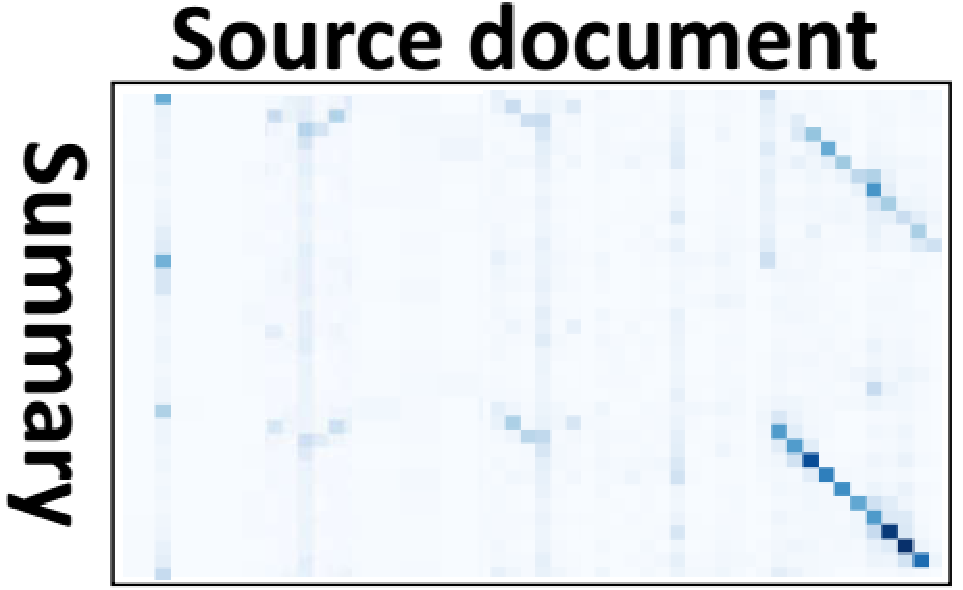
\includegraphics[width=0.16\linewidth]{mapITA}
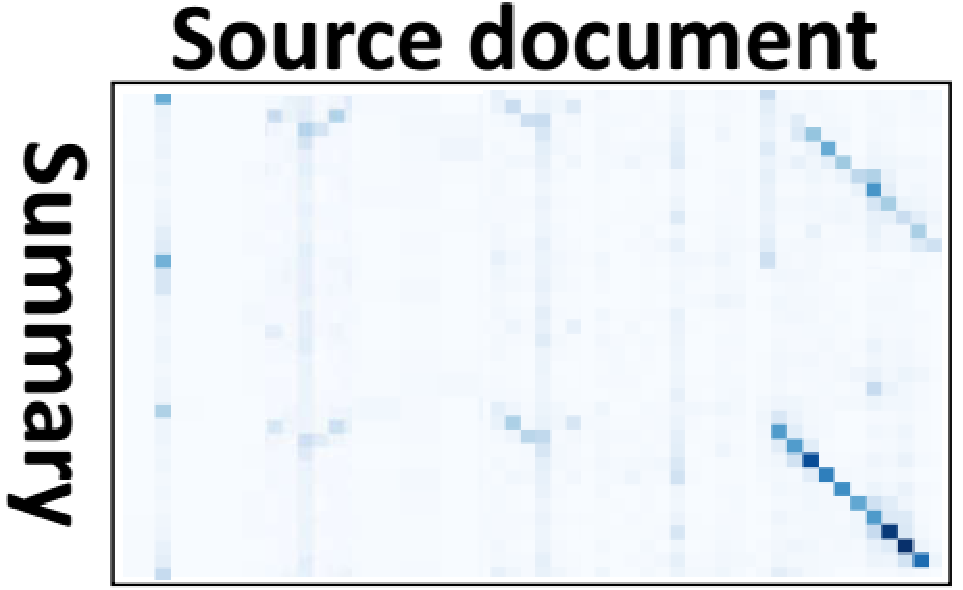
\includegraphics[width=0.26\columnwidth]{mapITA}
}
\quad
\subfigure[ITDA]{
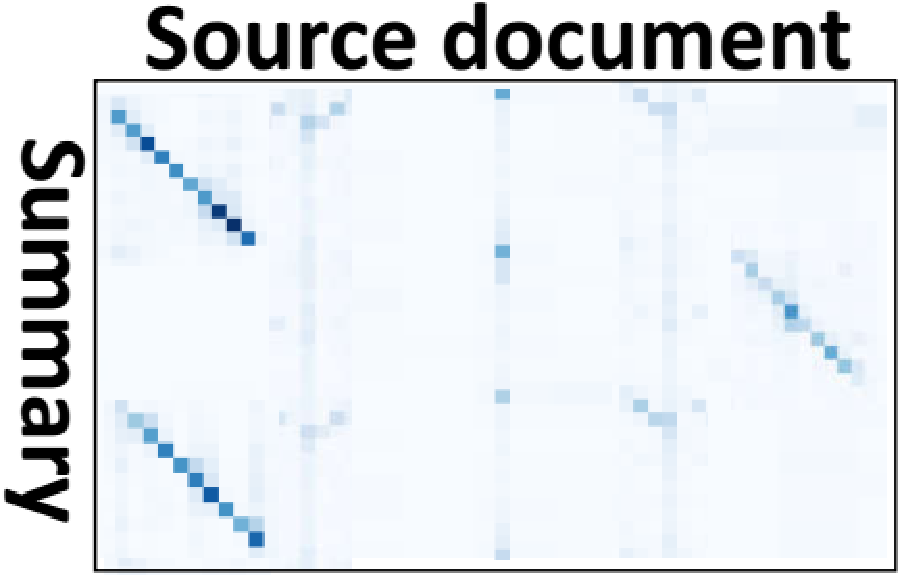
\includegraphics[width=0.26\linewidth]{mapITDA}
}
\quad
\subfigure[COV]{
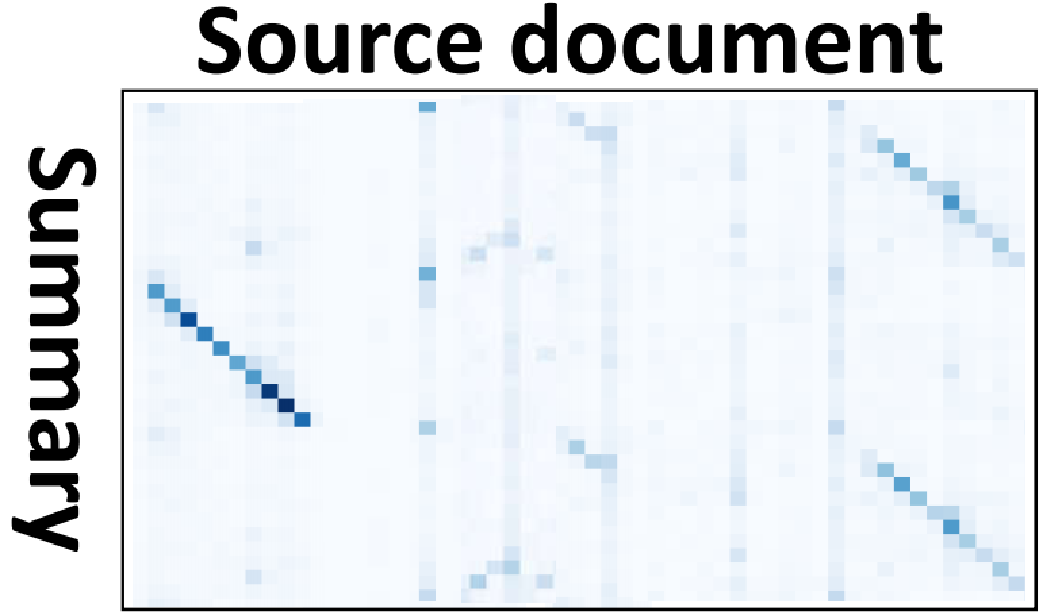
\includegraphics[width=0.26\linewidth]{mapCOV}
}
\quad
\subfigure[COVP]{
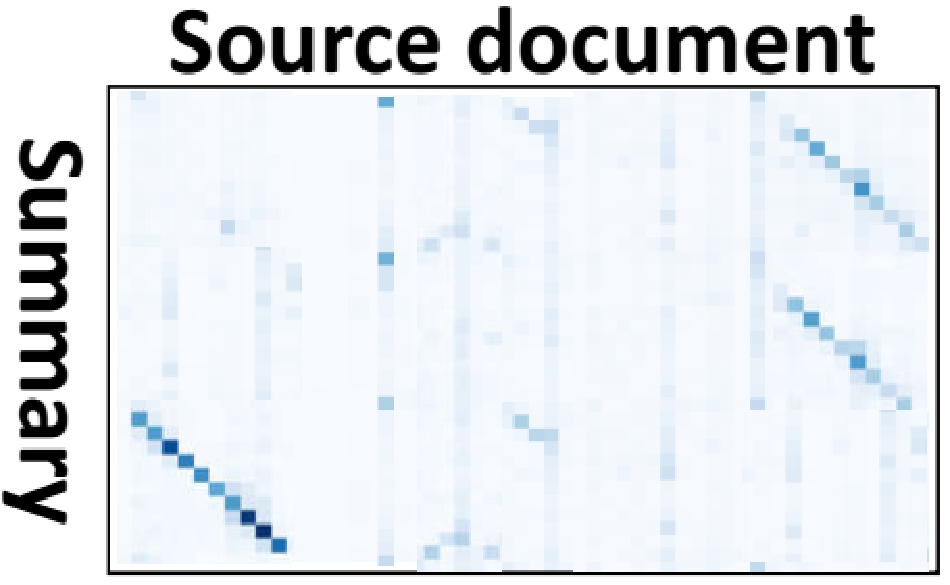
\includegraphics[width=0.26\linewidth]{mapCOVP}
}
\quad
\subfigure[SCL]{
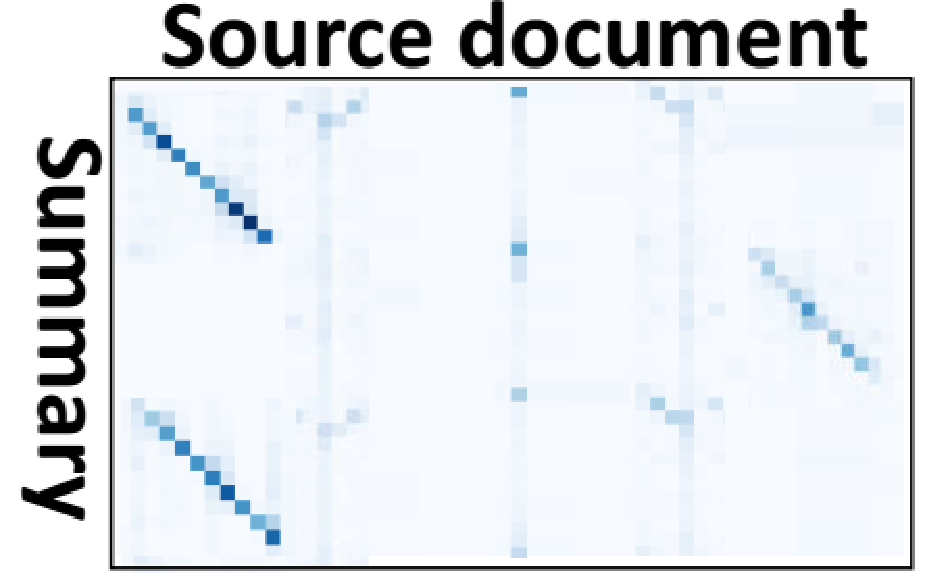
\includegraphics[width=0.26\linewidth]{mapSCL}
}
\quad
\subfigure[DivCNN]{
	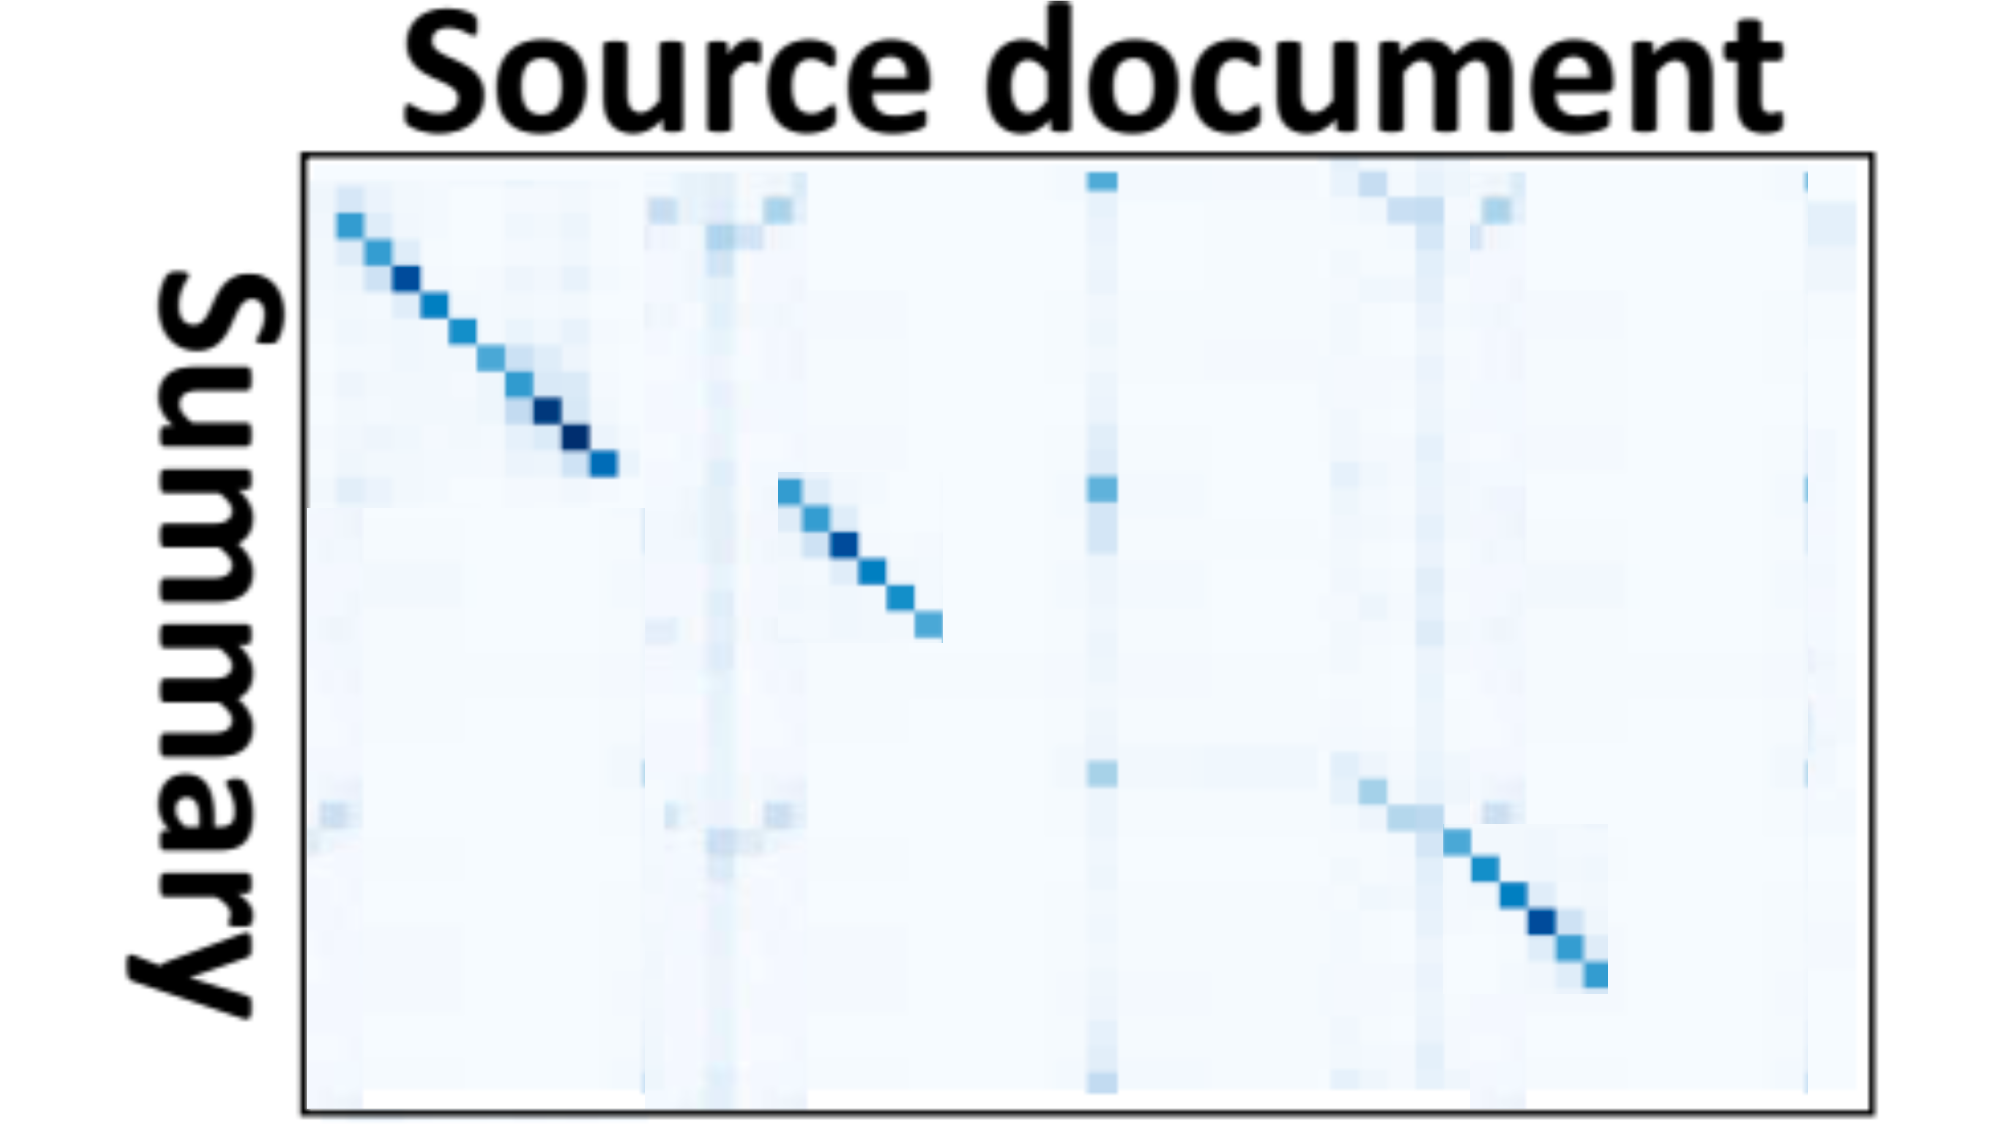
\includegraphics[width=0.26\linewidth]{mapDiv}
}
\quad
\subfigure[ATTF]{
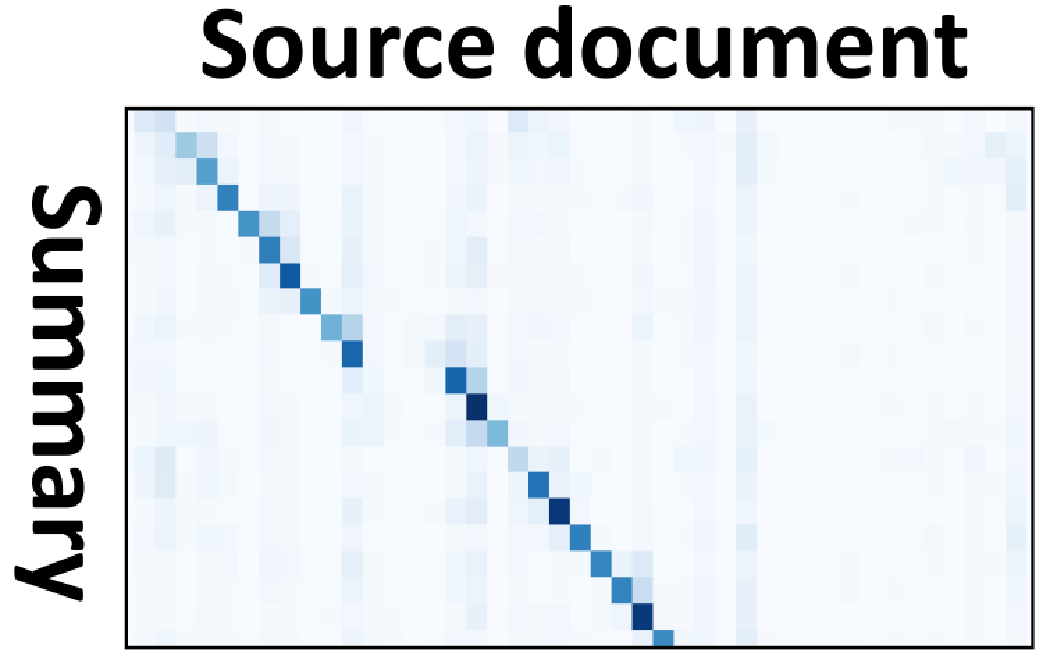
\includegraphics[width=0.26\linewidth]{map2}
}
\caption{Attention distribution of summaries for the source in \tabref{tab:example}}
\label{fig:attn_maps}
\end{figure}

Compared with the Gold standard,
ATTF still generates some repetitive sentences,
due to similar sentences in source
such as \exref{ex:repeatsrc}.
%The result of summarizing that document using ATTF and its local attention map are
The summary generated by ATTF and its local attention are
shown in \tabref{tab:src_rep} and \figref{fig:attn_map3}.
Also, SBD further reduces the repetition when combined with ATTF. 
%which demonstrates its effectiveness.

\begin{table}[th!]
\begin{center}
\caption{Summaries generated from \exref{ex:repeatsrc}.}
\begin{tabular}{|l|}%{|p{7cm}|rl|}
\hline \textbf{Reference:} oriol romeu is on a season-long loan at stuttgart from chelsea . \\
       the spanish midfielder predicts the scores in saturday 's matches . oriol goes \\
	   head-to-head with sportsmail 's martin keown .\\
\hline \textbf{ATTF:} chelsea beat manchester united on saturday . \textit{oriol romeu is currently} \\
       \textit{on a season-long loan at stuttgart . oriol romeu is currently on a season-long} \\
	   \textit{loan at bundesliga side stuttgart .}\\
\hline \textbf{SBD:} chelsea beat manchester united on saturday . chelsea face manchester \\
       united in the premier league . \\ 
\hline \textbf{ATTF+SBD:} chelsea face manchester united in the premier league on saturday . \\
       oriol romeu is currently on loan at stuttgart . \\
\hline
\end{tabular}
\end{center}
\label{tab:src_rep}
\end{table}

As shown in \tabref{tab:eval_repe}, TRI has the lowest total repeatedness score.
It does not generate any repetitive N-grams (N$>$2) and sentences 
because TRI prevents the generation of the same trigrams during testing.
But as the Gold row shows, reference summaries do have some natural repetition.
%As reference summaries are human written, 
Therefore we evaluate the correlation of repeatedness distribution between
generated summaries and reference summaries (\tabref{tab:eval_repcor}(a)).
Our proposed models perform best,
which indicates that ATTF and SBD are more capable of producing summaries with a natural level of repeatedness.
In addition, as shown in \tabref{tab:eval_repcor}(b), the correlations between the repeatedness and the human readability judgment are about 0.7, which means that the repeatedness score are useful. The repetition in summaries will affect coherence between sentences and the readability of summaries.
%It indicates that ATTF and SBD are more capable of producing summaries with a natural level of repeatedness.
%missing POIs and repetition in source documents.

\begin{table}[th!]
	\begin{center}
		\caption{Correlation Evaluation}
		\subtable[Repeatedness correlation between generated summaries and Gold summarie.]
		{
		\begin{tabular}{|l|c|c|c|}
			\hline
			& pearson  & spearman & kendall's tau \\
			\hline
			ATTF & \bf 1.0 & \bf 1.0 & \bf 1.0 \\
			TRI* & 1.0 & 0.89 & 0.84  \\
			SBD* & \bf 1.0 & \bf 1.0 & \bf 1.0 \\
			ATTF+TRI* & 1.0 & 0.89 & 0.84 \\
			ATTF+SBD* & \bf 1.0 & \bf 1.0 & \bf 1.0 \\
			\hline
		\end{tabular}
		}
		\qquad
		\subtable[the correlation between the repeatedness of the generated summaries and the human readibility judgement.]{
				\begin{tabular}{|l|c|c|c|}
				\hline
				& pearson  & spearman & kendall's tau \\
				\hline
				ATTF & 0.78 & 0.74 & 0.70 \\
				SBD* & 0.75 & 0.71 & 0.68 \\
				ATTF+SBD* & 0.75 & 0.74 & 0.69 \\
				\hline
			\end{tabular}
		}
        \label{tab:eval_repcor}
	\end{center}
\end{table}

\cut{%%%%%%5
\begin{table}[th!]
        \centering
        \caption{Repeatedness correlation between generated summaries and Gold summaries.}
        \begin{tabular}{|l|c|c|c|}
                \hline
                     & pearson  & spearman & kendall's tau \\
                \hline
                ATTF & \bf 1.0 & \bf 1.0 & \bf 1.0 \\
                TRI* & 1.0 & 0.89 & 0.84  \\
                SBD* & \bf 1.0 & \bf 1.0 & \bf 1.0 \\
                ATTF+TRI* & 1.0 & 0.89 & 0.84 \\
                ATTF+SBD* & \bf 1.0 & \bf 1.0 & \bf 1.0 \\
                \hline
        \end{tabular}
        \label{tab:eval_repcor}
\end{table}
}%%%%%%%%
\begin{figure}[th!]
\centering
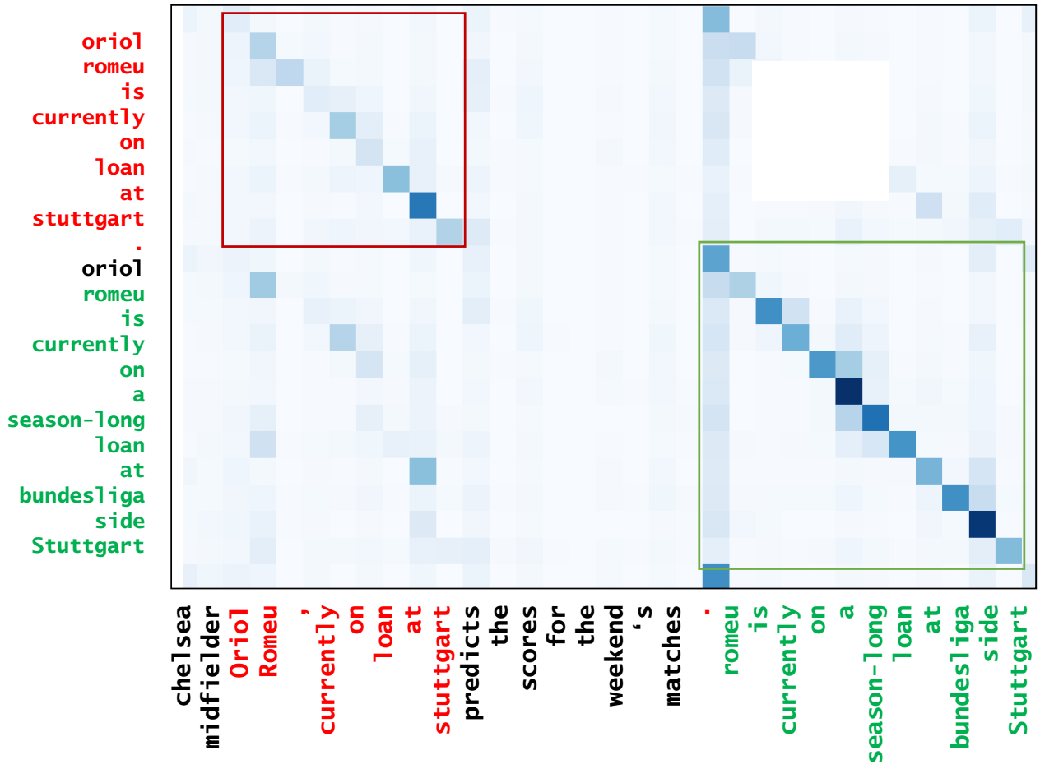
\includegraphics[width=0.84\columnwidth]{map3}
\caption{Attention distribution for ATTF in \tabref{tab:src_rep}}
\label{fig:attn_map3}
\end{figure}
	
\textbf{Readability.}
As shown in \tabref{tab:eval_repe}, 
the models with ATTF achieve the
%ATTF achieves the
highest readability score among all baselines, 
which means ATTF is more readable.
%without any operations during test.
As shown in \tabref{tab:eval_repe}(b),
TRI achieves the best score on repeatedness, 
% which represents the repetition over N-gram and sentences,
but lower readability score than other models.
The models with SBD are more readable than them with TRI. 
This is because that TRI interrupt the process of beam search through trigrams that cannot reflect the complete grammatical structure and semantic information. 
TRI always generates summaries with more grammatical and factural errors. 
SBD forbids the repetition at sentence-level during testing, which considers complete grammatical sturcture and semantic information.
As shown in \tabref{tab:strong_methods} and \tabref{tab:sbd_exp}, SBD weakens the influence of the meddling of beam search during generation
and generates more readable summaries.
The higher ROUGE scores shows that SBD enhances performance of CNN and ATTF by reducing the repetitive unreadable sentences. 
%All of our models score higher than $0.80$. 

\cut{%%%%%%%%%
\begin{table}[th!]
	\centering
	\begin{tabular}{|l|c|c|c|}
		\hline
		     & pearson  & spearman & kendall's tau \\
		\hline
		TRI* & 1.0 & 0.894 & 0.837  \\
		SBD* & 1.0 & 1.0 & 1.0 \\
		ATTF+TRI* & 1.0 & 0.894 & 0.837 \\
		ATTF+SBD* & \bf 1.0 & \bf 1.0 & \bf 1.0 \\
		\hline
	\end{tabular}
    \caption{Repeatedness correlation between generated summaries and Gold summaries.}
	\label{tab:eval_repcor}
\end{table}
}%%%


\textbf{Speed.} 
We compare the speed of our model to RNN~\citep{SeeLM17} and Transformer-large~\citep{Attn17}
which used K40. 
We perform experiments on GTX-1080ti and scale the speed 
reported for the RNN methods,
since GTX-1080ti is twice as fast as K40~\citep{gehring2017convs2s}.
The training speed and testing speed of CNN+ATTF 
is faster than RNN seq2seq model and Transformer
as CNN can be trained in parallel and ATTF .
The gap of training/testing time between ATTF and Transformer is not much large,
but the memory usage of Transformer is much larger than ATTF.
Because Transformer has more trainable parameters than ATTF.

The convergence rate of models with ATTF depends on three aspects:
{\em dataset}, {\em basic model} and {\em experimental settings}.
For {\em dataset}, ATTF redistributs the attention distribution between source documents and summaries during decoding,
which dynamically searches the attended segment in source by the predicted segments in summary.
Thus, the convergence rate of the models with ATTF depends on the length of source documets and summaries.
The ATTF applied on better {\em basic models} converges faster,
because better basic models learn the alignment between source documents and summaries better.
The {\em experimental setting} also impacts the convergence rate of the model with ATTF.
At the beginning of training, a large learning rate makes the model converge faster. 
When most of the samples have been trained, 
the model converges rapidly by decreasing the learning rate.
%generate summaries much faster than previous RNN seq2seq models. 

As shown in \tabref{tab:eval_main} and \tabref{tab:eval_speed}, 
SBD is the best sentence-level backtracking decoder.
Compared with SBD-b1 and SBD-b2,
SBD logs higher ROUGE scores without losing much on speed. 
ATTF+SBD achieves the best ROUGE scores 
and its training time and testing time do not increase too much.

\begin{table}[th!]
\centering
\caption{Time and speed of training and testing. The training time of the model with SBDs
is empty because SBDs are only used during testing.}
\begin{tabular}{|l|c|c|c|c|}
\hline
\multirow{2}{*}{Model} & Train & \multicolumn{3}{|c|}{Test} \\
\cline{2-5}
& Time (h) & Time (s) & summaries/s & tokens/s \\
\hline
RNN  & 336.54 &21600 & 0.48 & 29.60 \\
Transformer & 115.44 & 2094.64 & 5.65 & 214.83 \\
\hline
CNN & 48.3 &346.1 & 30.36 & 1343.46 \\
SBD-b1 & - & 412.8 & 25.46 & 1126.38 \\
SBD-b2 & -  &843.5 &12.16 & 551.24 \\
SBD & - &912.8 & 11.51 & 493.68 \\
ATTF & 108 &1332 & 7.89 &  349.00 \\
ATTF+SBD & - &1832.3 & 5.74 &  253.77 \\
\hline
\end{tabular}
\label{tab:eval_speed}
\end{table}

\textbf{Generalization.} 
\tabref{tab:generalization} shows the generalization of our abstractive system to other two datasets, Newsroom and DUC 2002, where our
proposed models achieve better scores than vanilla CNN seq2seq model in terms of ROUGE scores, readability and repeatedness. 
We use the same settings of $\beta=3$ ($sz$ in previous version) in Section 2.2 and $n=5$ in Eq.(11), because the proportion of seqments with length greater than 3 and reference summaries with LCS greater than 5 were about 90\%. As show in , our proposed models can be better generalization on other datasets about news, along with repetition reduction and the improvement of readability.
This shows that our proposed models can be generalized well.
\begin{table}[th!]
	\begin{center}
		\caption{ROUGE scores, total repeatedness (Rep) and readability of models on Newsroom and DUC}
		\begin{tabular}{|l|c|c|c|c|c|c|c|c|c|c|}
			\hline
			\multirow{2}{*}{Model} & \multicolumn{5}{|c|}{Newsroom} &\multicolumn{5}{|c|}{DUC} \\
			\cline{2-11}
			&R-1 & R-2 & R-L& Rep & Readable &R-1 & R-2 & R-L & Rep & Readable\\
			\hline
			CNN &  27.43 & 18.62 & 26.77 & 20.38 & 2.65 & 26.02 & 8.76 & 22.05& 19.32 & 2.32 \\
            SBD &  28.2 & 20.17 & 26.94 & 0.62 & 3.02 & 26.86 & 9.27 & 22.75& 0.43 & 2.85 \\
            ATTF &  28.43 & 20.05 & 27.32 & 15.32 & 3.42 & 26.94 & 9.05 & 22.33& 17.16 & 3.11 \\
			ATTF+SBD &  \bf 28.93& \bf 21.46 & \bf 27.55 & \bf 0.58 & \bf 3.73 & \bf 27.02 & \bf 9.56 & \bf 23.05& \bf 0.40 & \bf 3.5 \\
			\hline
		\end{tabular}
		\label{tab:generalization}
	\end{center}
\end{table}


%\subsection{Significance Test on ROUGE scores}
\textbf{Significance Test.} We use significance test to prove that the ROUGE scores in \tabref{tab:eval_main} is reliable.
We take t-test 
\citep{loukina2014automatic,albert2017exploring}
as our significance test to
measure that the ROUGE scores between our proposed approach (ATTF+SBD) and each baseline are significant or not. 
As shown in \tabref{tab:ttest},
all p-values are less than 0.05. 
The smaller p-value, the higher significant.
Thus, the difference of the similarity results is significant. 
\begin{table}[th!]
	\begin{center}
		\caption{p-value of significance test between 
			our best proposed model (ATTF+SBD) and baselines on ROUGE scores}
		\begin{tabular}{|l|c|c|c|}
			\hline
			Model &   R-1 & R-2 & R-L \\
			\hline
			CNN &  2.32e-35 & 6.34e-48 & 3.68e-10 \\
			ITA &  6.14e-34 & 2.12e-48 & 5.67e-12 \\
			ITDA & 2.76e-32 & 4.52e-44 & 3.94e-12 \\
			COV	& 4.14e-30 & 4.61e-50 & 7.12e-12 \\
			COVP & 2.51e-32 & 3.17e-41 & 2.15e-10 \\
			SCL	& 3.11e-32 & 3.29e-44 & 3.43e-15 \\
			DivCNN	& 2.28e-31 & 4.27e-40 & 6.81e-10 \\
			TRI & 5.25e-30 & 1.33e-43 & 3.67e-12 \\
			\hline
		\end{tabular}
		\label{tab:ttest}
	\end{center}
\end{table}

Overall, the summaries generated by sequence-to-sequence models with attention mechanism always contain repetition.  
Through our observations, there are two reasons for repetition in abstractive summarization.
One is that the traditional attention mechanisms attend to the same location in source document at decoding.
The other is that the attention mechanism attend to the repetitive sentences in different locations in source document. 
As shown in \figref{fig:attn_maps} and \tabref{tab:src_rep},
our proposed ATTF and SBD effectively solve above two problems.  
As ATTF deals with incorrect attention distribution
between the inputs of encoder and decoder to 
reduce repetition in generated summaries,
the seq2seq models with attention mechanism between encoder and decoder
can be improved via ATTF.
The SBD can only be used at testing, which is suitable for the models with decoder.
Since RNN-based and transformer-based seq2seq models,
including attention mechanism between encoder and decoder,
always suffer from repetition in generated summaries, 
we can reasonably deduce that these models will benefit from our proposed ATTF and SBD as well.
The higher ROUGE scores (\tabref{tab:eval_main}) of our model means that
the summaries generated by our model are more similar to their corresponding reference summaries.
The natural-level repeatedness and higher readability score (\tabref{tab:eval_repe}) of our model means 
that our model can produce summaries with higher quality.
ATTF is applied to the attention mechanism between encoder and decoder,
which impacts the time of decoding at training and testing.
SBD only impacts the time of decoding during test.
%So ATTF+SBD makes the models slowdown in different degrees 
%because of different time costs for encoding.
%The more time the encoder takes, the less the model slow down.
ATTF+SBD takes about the same amount of time for additional models to slow down.
For RNNs and transformers, after adding ATTF+SBD,
there would be less than 6 times slowdown
(As shown in Table 11, for the vanilla CNN, there is a roughly 6 times slowdown after adding ATTF+SBD.)
since RNNs and transformers spend more training time and testing time on encoding than CNN.
As a result, our model can improve the reading speed and accuracy of reading comprehension.


